% Licence, CC-BY
% This template borrowed from Karthik Ram, for Berkeley-ifcation of the Amsterdam theme.
\documentclass{beamer}\usepackage[]{graphicx}\usepackage[]{color}
%% maxwidth is the original width if it is less than linewidth
%% otherwise use linewidth (to make sure the graphics do not exceed the margin)
\makeatletter
\def\maxwidth{ %
  \ifdim\Gin@nat@width>\linewidth
    \linewidth
  \else
    \Gin@nat@width
  \fi
}
\makeatother

\definecolor{fgcolor}{rgb}{0.345, 0.345, 0.345}
\newcommand{\hlnum}[1]{\textcolor[rgb]{0.686,0.059,0.569}{#1}}%
\newcommand{\hlstr}[1]{\textcolor[rgb]{0.192,0.494,0.8}{#1}}%
\newcommand{\hlcom}[1]{\textcolor[rgb]{0.678,0.584,0.686}{\textit{#1}}}%
\newcommand{\hlopt}[1]{\textcolor[rgb]{0,0,0}{#1}}%
\newcommand{\hlstd}[1]{\textcolor[rgb]{0.345,0.345,0.345}{#1}}%
\newcommand{\hlkwa}[1]{\textcolor[rgb]{0.161,0.373,0.58}{\textbf{#1}}}%
\newcommand{\hlkwb}[1]{\textcolor[rgb]{0.69,0.353,0.396}{#1}}%
\newcommand{\hlkwc}[1]{\textcolor[rgb]{0.333,0.667,0.333}{#1}}%
\newcommand{\hlkwd}[1]{\textcolor[rgb]{0.737,0.353,0.396}{\textbf{#1}}}%

\definecolor{shadecolor}{rgb}{.97, .97, .97}
\definecolor{messagecolor}{rgb}{0, 0, 0}
\definecolor{warningcolor}{rgb}{1, 0, 1}
\definecolor{errorcolor}{rgb}{1, 0, 0}

\setbeamertemplate{frametitle}[default][center]
\setcounter{secnumdepth}{-1}
\usetheme{Amsterdam}


\usepackage{tikz}

% --------------------------------------------------------------
\begin{document}
\title{Update On ATWS Studies}
\author[Kathryn D. Huff]{
\includegraphics[height=2cm]{bk}\\Kathryn D.  Huff}
\maketitle

\section{Motivation}
% Waste is a problem
% Decisionmakers are contemplating many fuel cycle options
% Decisionmakers are contemplating many repository options
% Interfacing between FCO/SA campaign and UFD campaign

\begin{frame}[ctb!]
  \frametitle{Future Disposal System Options}
   \begin{minipage}{0.44\textwidth}
     \begin{figure}[h!]
         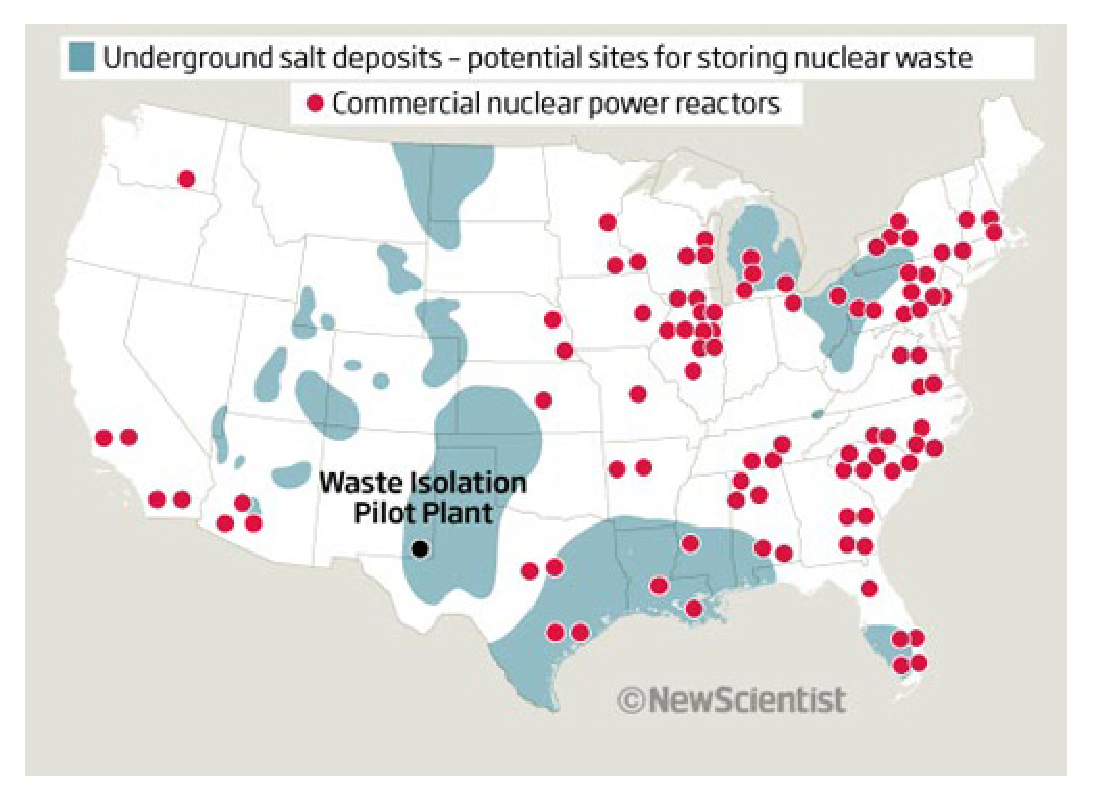
\includegraphics[width=0.8\textwidth]{cyder/images/saltNewScientist.eps}
         \caption{U.S. Salt Deposits, ref. \cite{newscientist_where_2011}.}
     \end{figure}
     \begin{figure}[h!]
         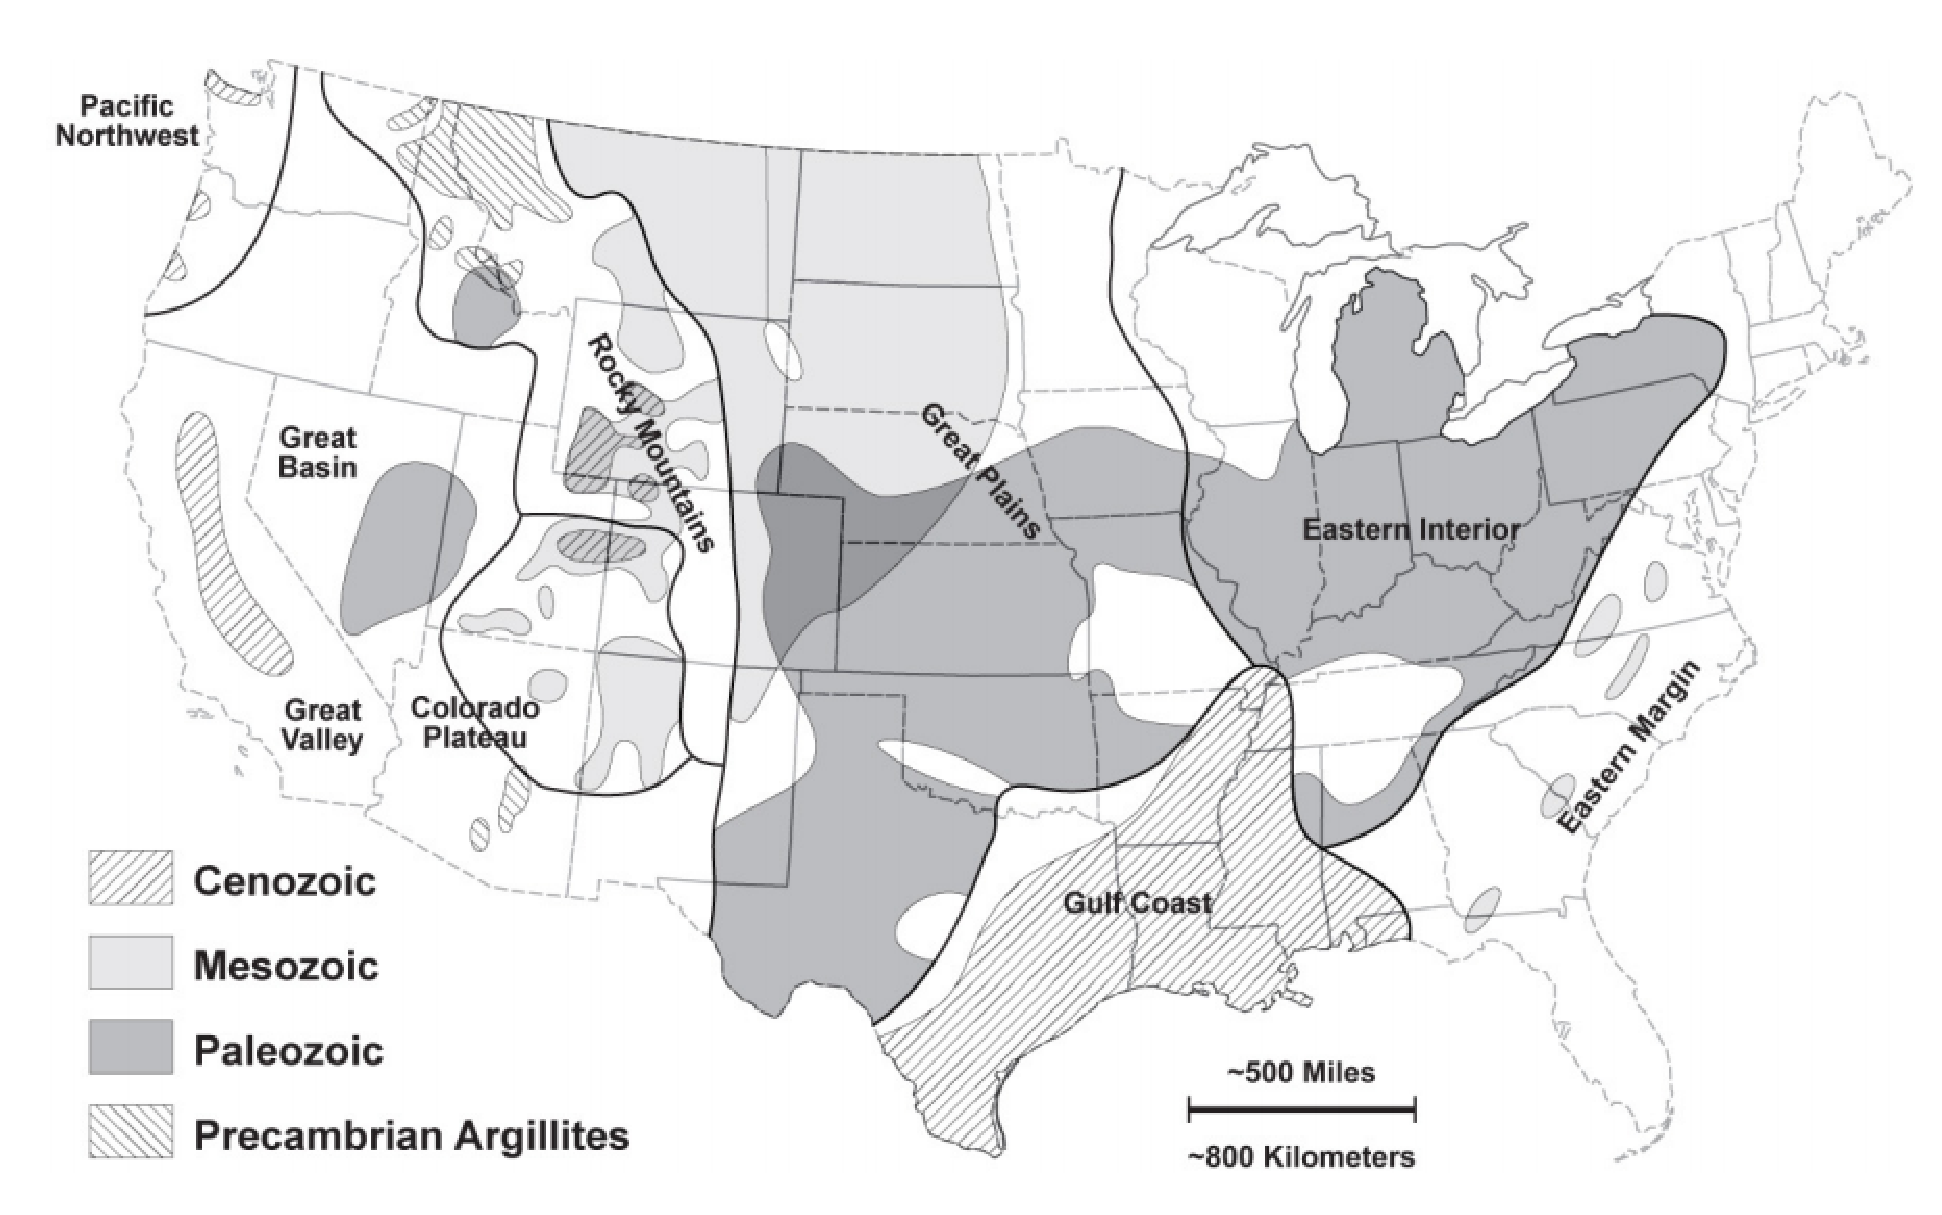
\includegraphics[width=0.8\textwidth]{cyder/images/clayGonzales.eps}
         \caption{U.S. Clay Deposits, ref. \cite{gonzales_shales_1985}.}
     \end{figure}
   \end{minipage}
   \hspace{0.01cm}
   \begin{minipage}{0.44\textwidth}
     \begin{figure}[h!]
         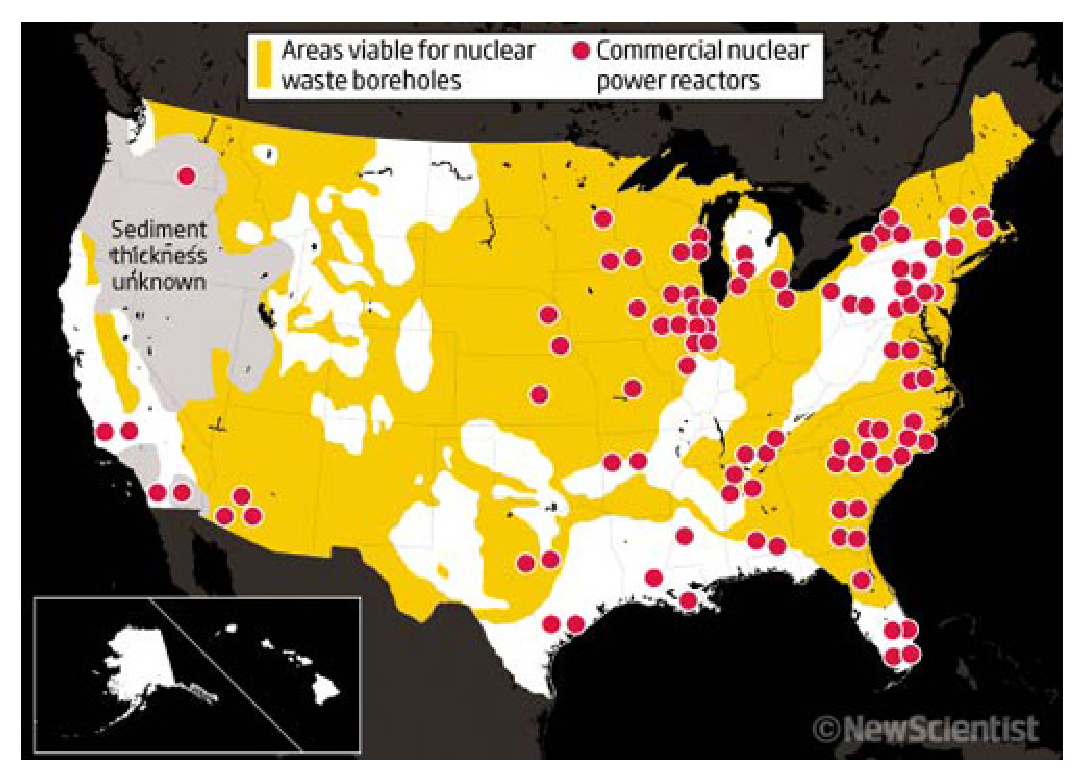
\includegraphics[width=0.8\textwidth]{cyder/images/boreholeNewScientist.eps}
         \caption{U.S. Crystalline Basement, ref.  \cite{newscientist_where_2011}.}
     \end{figure}
     \begin{figure}[h!]
         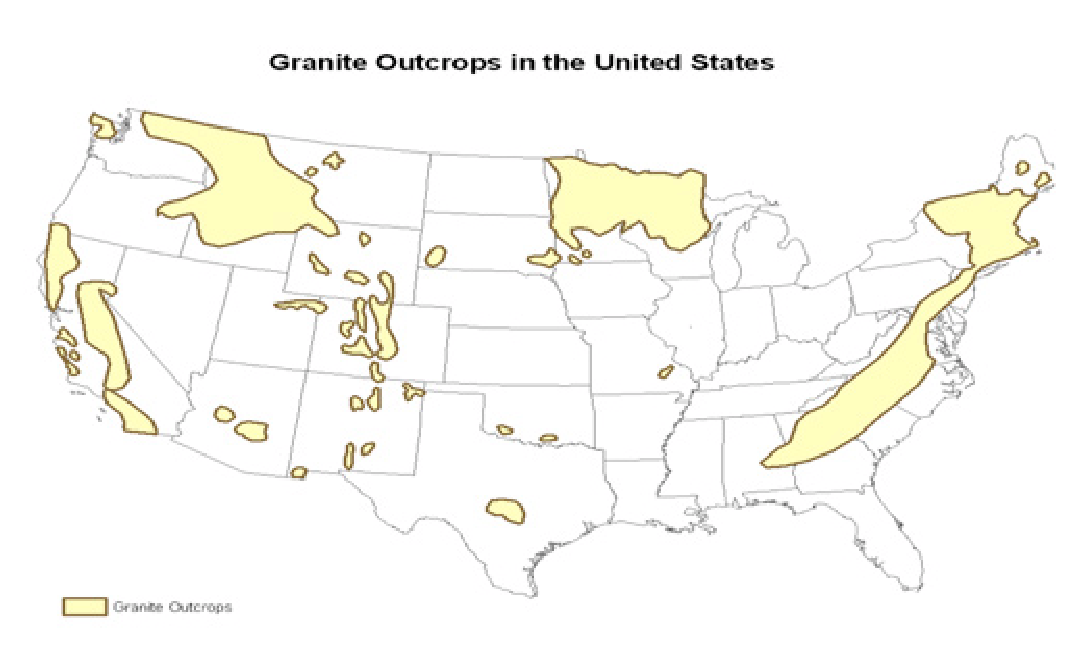
\includegraphics[width=0.8\textwidth]{cyder/images/graniteBush.eps}
         \caption{U.S. Granite Beds, ref. \cite{bush_economic_1976}.}
     \end{figure}
   \end{minipage}
\end{frame}


\begin{frame}[ctb!]
  \frametitle{Future Fuel Cycle Options}
       % Future Fuel Cycles
    \begin{table}
      \centering
      \footnotesize{
      \begin{tabular}{|l|l|l|}
        \multicolumn{3}{c}{\textbf{Domestic Fuel Cycle Options}}\\
        \hline
        Title & Description& Challenges \\
        \hline
        \hline
        Open          & Once Through         & High Temperatures, Volumes \\
                      & Current US PWR Fleet &      \\
                      & No Separations       &      \\
                      & No Recycling         &      \\
                      & Higher Burnups &      \\
        \hline
        Modified Open & Partial Recycling    & Both high volumes and myriad fuel streams \\
                      & Next Gen. PWR Fleet &      \\
                      & Limited Separations  &      \\
                      & Limited Transmutation &      \\
                      & Advanced Fuel Forms  &      \\
                      & HLW treatment    &          \\
        \hline
        Closed        & Full Recycling       & Myriad fuel streams \\
                      & Full Separations &      \\
                      & Full Recycling &      \\
                      & VHTGR, SFRs, &      \\
                      & other transmutation & \\
                      & HLW treatment  &      \\
        \hline
      \end{tabular}
      \caption[Fuel Cycle Options]{Domestic Fuel Cycle Options }
      \label{tab:fco}
      }
    \end{table}

\end{frame}



\section{Prior Art}
% --------------------------------------------------------------
\begin{frame}[fragile]
  \frametitle{Previous Work}
  \begin{itemize}
    \item Oak Ridge AHTR - unnecessary (Varma, Holcomb, et al.)
    \item COMSOL TH response analysis (Huff, Scarlat)
    \item Algebraic, 1-group LOFC neutronics analysis (Cisneros)
    \item Algebraic, 1-group RIA neutronics analysis (Greenspan, Fratoni)
  \end{itemize}

\end{frame}

% --------------------------------------------------------------
\begin{frame}[fragile]
  \frametitle{Design Point?}
  \begin{figure}[htbp!]
    \begin{center}
      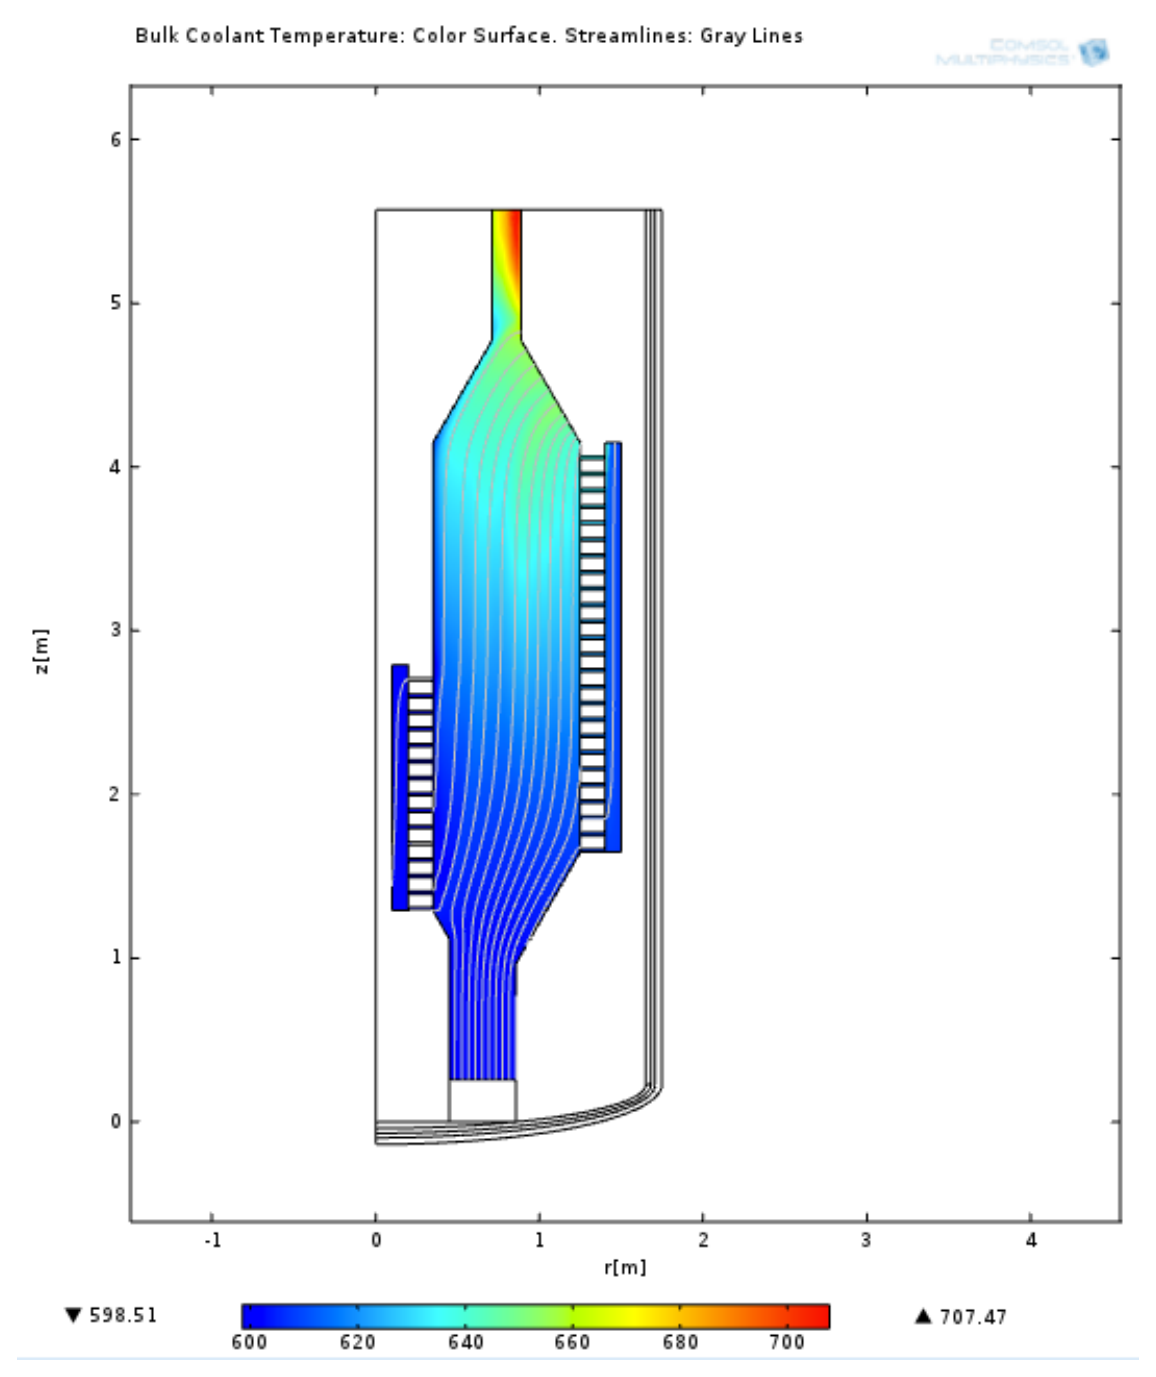
\includegraphics[height=0.8\textheight]{./priorart/coolant_temps_100_deg_rise.eps}
    \end{center}
    \caption{For 100 degree temperature rise design point across the core.}
    \label{fig:200degrise}
  \end{figure}
\end{frame}

% --------------------------------------------------------------
\begin{frame}[fragile]
  \frametitle{Design Point?}

  \begin{figure}[htbp!]
    \begin{center}
      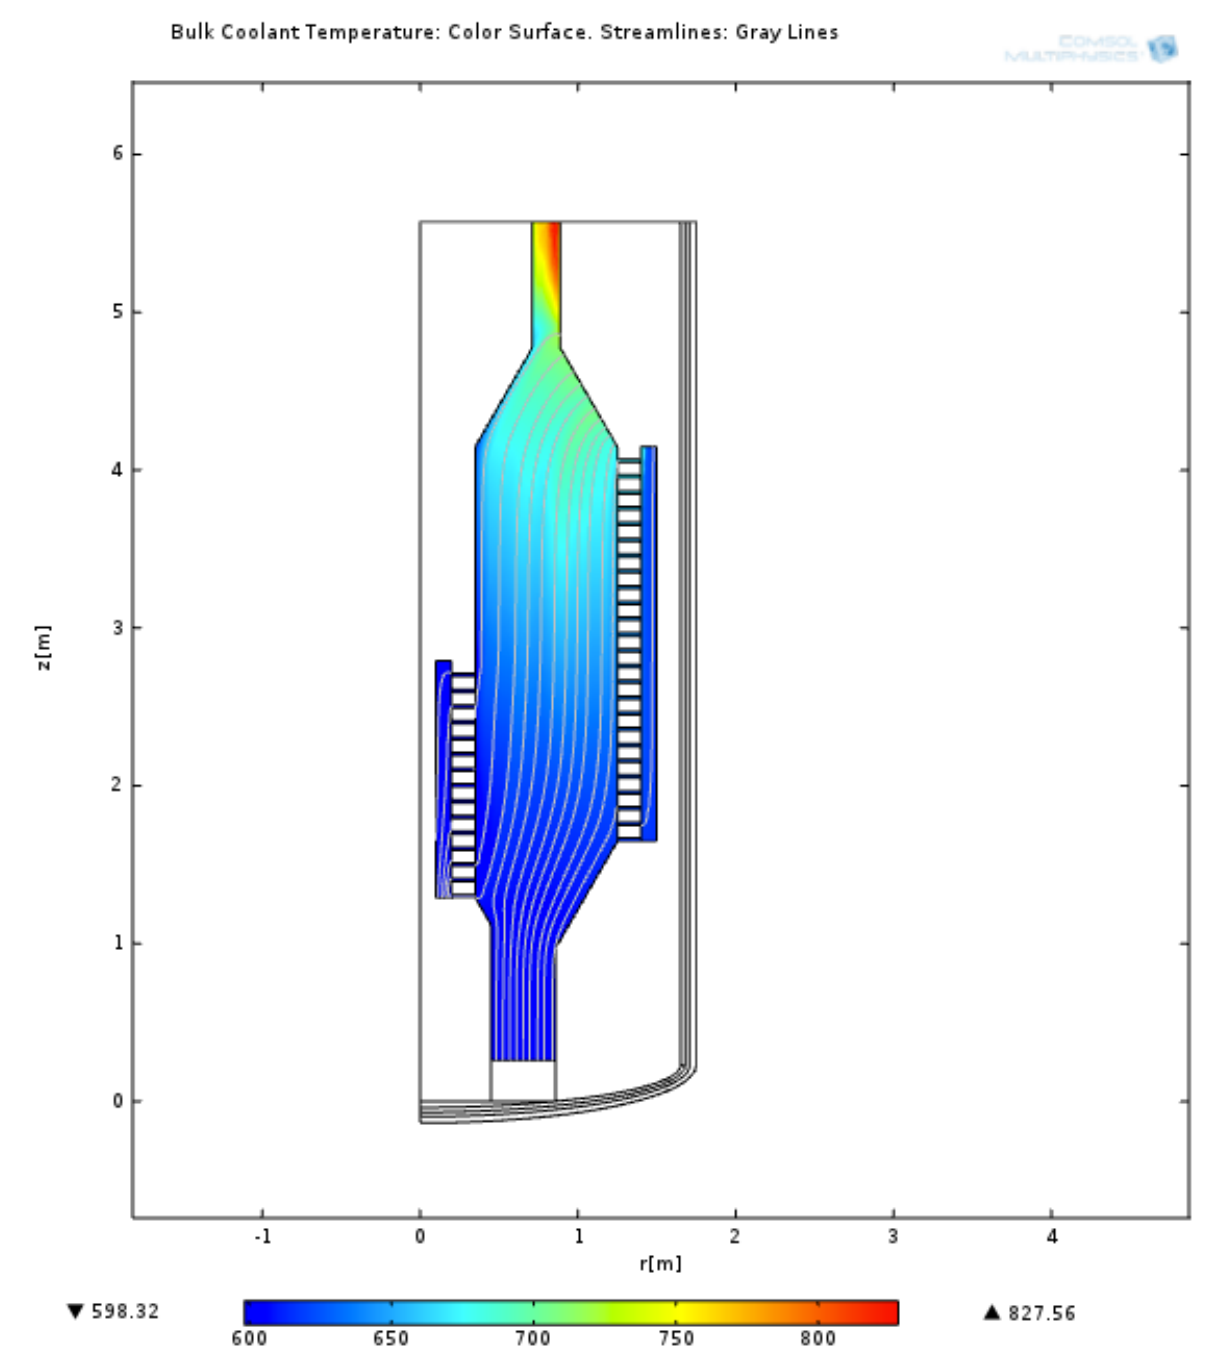
\includegraphics[height=0.8\textheight]{./priorart/coolant_temps_200_deg_rise.eps}
    \end{center}
    \caption{For 200 degree temperature rise design point across the core.}
    \label{fig:200degrise}
  \end{figure}
\end{frame}


\section{Approach}
% --------------------------------------------------------------
\begin{frame}[fragile]
  \frametitle{Approach}
  \begin{itemize}
    \item Collect data
    \item Develop 0D coupled neutronics/TH model (PyRK)
    \item Compare to algebraic results
    \item Develop 3D neutronics/TH model
    \item Compare 0D and 3D models
    \item Connect additional coupled physics
  \end{itemize}

\end{frame}

\section{Progress}


% --------------------------------------------------------------
\begin{frame}[fragile]
  \frametitle{Recent Progress}
  \begin{itemize}
    \item 1-D, 6 group neutronics model
    \item 1-D thermal hydraulics model
    \item Forward Difference Coupling 
    \item 3-D Mesh Development
  \end{itemize}
\end{frame}

% --------------------------------------------------------------
\begin{frame}[fragile]
  \frametitle{Coupled Kinetics}
  \footnotesize{
\begin{equation} 
  \frac{d}{dt}\left[
    \begin{array}{c}
      p\\
      \zeta_1\\
      .\\
      .\\
      .\\
      \zeta_J\\
      \omega_1\\
      .\\
      .\\
      .\\
      \omega_K\\
      T_{fuel}\\
      T_{cool}\\
      .\\
      .\\
      .\\
    \end{array}
    \right]
    =
    \left[
      \begin{array}{ c }
        \frac{\rho(t,T_{fuel},T_{cool},\cdots)-\beta}{\Lambda}p + 
        \displaystyle\sum^{j=J}_{j=1}\lambda_j\zeta_j\\
        \frac{\beta_1}{\Lambda} p - \lambda_1\zeta_1\\
        .\\
        .\\
        .\\
        \frac{\beta_J}{\Lambda}p-\lambda_J\zeta_J\\
        \kappa_1p - \lambda_1\omega_1\\
        .\\
        .\\
        .\\
        \kappa_{k p} - \lambda_k\omega_{k}\\
        f(p, C_p^{fuel}, T_{fuel}, T_{cool},\cdots)\\
        g(C_p^{cool}, T_{fuel}, T_{cool},\cdots)\\
        .\\
        .\\
        .\\
      \end{array}
      \right]
      \label{eqn:ourPRKE}
    \end{equation}
  
  }
\end{frame}

% --------------------------------------------------------------
\begin{frame}[fragile]
  \frametitle{Coupled Kinetics}
  \footnotesize{
\begin{equation} 
  \frac{d}{dt}\left[
    \begin{array}{c}
      p\\
      \zeta_1\\
      .\\
      .\\
      .\\
      \zeta_J\\
      \omega_1\\
      .\\
      .\\
      .\\
      \omega_K\\
      \textcolor{red}{T_{fuel}}\\
      \textcolor{red}{T_{cool}}\\
      .\\
      .\\
      .\\
    \end{array}
    \right]
    =
    \left[
      \begin{array}{ c }
        \frac{\textcolor{red}{\rho(t,T_{fuel},T_{cool},\cdots)}-\beta}{\Lambda}p + 
        \displaystyle\sum^{j=J}_{j=1}\lambda_j\zeta_j\\
        \frac{\beta_1}{\Lambda} p - \lambda_1\zeta_1\\
        .\\
        .\\
        .\\
        \frac{\beta_J}{\Lambda}p-\lambda_J\zeta_J\\
        \kappa_1p - \lambda_1\omega_1\\
        .\\
        .\\
        .\\
        \kappa_{k p} - \lambda_k\omega_{k}\\
        f(p, C_p^{fuel}, T_{fuel}, T_{cool},\cdots)\\
        g(C_p^{cool}, T_{fuel}, T_{cool},\cdots)\\
        .\\
        .\\
        .\\
      \end{array}
      \right]
      \label{eqn:ourPRKE}
    \end{equation}
  
  }
\end{frame}



% --------------------------------------------------------------
\begin{frame}[fragile]
  \frametitle{Neutronics Block}
  \footnotesize{
\begin{equation} 
  \frac{d}{dt}\left[
    \begin{array}{c}
      p\\
      \zeta_1\\
      .\\
      .\\
      .\\
      \zeta_J\\
      \omega_1\\
      .\\
      .\\
      .\\
      \omega_K\\
    \end{array}
    \right]
    =
    \left[
      \begin{array}{ c }
        \frac{\rho(t,T_{fuel},T_{cool},\cdots)-\beta}{\Lambda}p + 
        \displaystyle\sum^{j=J}_{j=1}\lambda_j\zeta_j\\
        \frac{\beta_1}{\Lambda} p - \lambda_1\zeta_1\\
        .\\
        .\\
        .\\
        \frac{\beta_J}{\Lambda}p-\lambda_J\zeta_J\\
        \kappa_1p - \lambda_1\omega_1\\
        .\\
        .\\
        .\\
        \kappa_{k}p - \lambda_k\omega_{k}\\
      \end{array}
      \right]
      \label{eqn:ourPRKE}
    \end{equation}
  
  }
\end{frame}

% --------------------------------------------------------------
\begin{frame}[fragile]
  \frametitle{Neutronics Data Needs}
\footnotesize{
  \begin{align}
    \rho(t,&T_{fuel},T_{cool},T_{mod}, T_{refl}) = \mbox{ reactivity, [pcm]}\\
    \beta &= \mbox{ fraction of neutrons that are delayed}\\ 
    \beta_j &= \mbox{ fraction of delayed neutrons from precursor group j}\\  
    \zeta_j &= \mbox{ concentration of precursors of group j}\\ 
    \lambda^{d}_j &= \mbox{ decay constant of precursor group j}\\ 
    \Lambda &= \mbox{ mean generation time ? }\\
    \omega_k &= \mbox{ decay heat from FP group k}\\ 
    \kappa_k &= \mbox{ heat per fission for decay FP group k}\\ 
    \lambda^{FP}_k &= \mbox{ decay constant for decay FP group k} 
  \end{align}
}

\end{frame}
% --------------------------------------------------------------
\begin{frame}[fragile]
  \frametitle{Neutronics Data : Delayed Neutron Model}

    \begin{table}
      \begin{tabular}{|l|c|c|c|c|}
        \hline
        j & $t_{1/2}$ & $\lambda^d_j$  & $\eta_j$ & $\beta_j$\\
          &   $[s]$   &    $[1/s]$     & $[n/f]$  & \\
        \hline
        1   &  $ 55.72 $  &  $ 0.0124 $  &  $ 0.00052 $  &  $ 0.000215$  \\
        2   &  $ 22.72 $  &  $ 0.0305 $  &  $ 0.00546 $  &  $ 0.001424$  \\
        3   &  $ 6.22  $  &  $ 0.111  $  &  $ 0.00310 $  &  $ 0.001274$  \\
        4   &  $ 2.30  $  &  $ 0.301  $  &  $ 0.00624 $  &  $ 0.002568$  \\
        5   &  $ 0.614 $  &  $ 1.14   $  &  $ 0.00182 $  &  $ 0.000748$  \\
        6   &  $ 0.230 $  &  $ 3.01   $  &  $ 0.00066 $  &  $ 0.000273$  \\
        \hline
      \end{tabular}
      \caption{Delayed neutron data Decay heat data, $^{235}$U thermal fission. 
    Lamarsh.}
      \label{tab:delayedneutrons}
    \end{table}

\end{frame}

% --------------------------------------------------------------
\begin{frame}[fragile]
  \frametitle{Neutronics Data : Decay Heat Model}
    \begin{table}
      \begin{tabular}{|l|c|c|}
        \hline
        k & $\lambda^{FP_k}$ & $\kappa_k$\\
                          &  $[1/s]$         & $[MeV/fission-s]$ \\
        \hline
        1   &  $ 6.587\times10^{  0} $  &  $ 2.658\times10^{  0}$ \\
        2   &  $ 1.490\times10^{ -1} $  &  $ 4.619\times10^{ -1}$ \\
        3   &  $ 2.730\times10^{ -1} $  &  $ 6.069\times10^{ -2}$ \\
        4   &  $ 2.173\times10^{ -2} $  &  $ 5.593\times10^{ -3}$ \\
        5   &  $ 1.961\times10^{ -3} $  &  $ 6.872\times10^{ -4}$ \\
        6   &  $ 1.025\times10^{ -4} $  &  $ 6.734\times10^{ -5}$ \\
        7   &  $ 4.923\times10^{ -6} $  &  $ 6.413\times10^{ -6}$ \\
        8   &  $ 2.679\times10^{ -7} $  &  $ 6.155\times10^{ -7}$ \\
        9   &  $ 1.452\times10^{ -8} $  &  $ 8.288\times10^{ -8}$ \\
       10   &  $ 1.893\times10^{ -9} $  &  $ 1.923\times10^{ -8}$ \\
       11   &  $ 1.633\times10^{-10} $  &  $ 1.214\times10^{ -9}$ \\
       \hline
      \end{tabular}
      \caption{Decay heat data, ANS/ANSI 5.1-1971 for $^{235}$U thermal fission.}
      \label{tab:decayheat}
    \end{table}

\end{frame}

% --------------------------------------------------------------

\begin{frame}[fragile]
  \frametitle{Neutronics Data : Reactivity Coefficients}
    \begin{table}
      \begin{tabular}{|l|c|c|c|}
        \hline
        Component & $T_{0}$  &  $T_0$ & $\frac{\partial\alpha}{\partial T}$\\
                  & $[K]$    &  $[K]$ & $[pcm/K]$ \\
        \hline
        fuel  & 730 & 1003.15 & -3.8 \\
        cool  & 650 &  923.15 & -1.8 \\
        mod   & 700 &  973.15 & -0.7 \\
        refl  & 650 &  923.15 &  \textcolor{red}{1.8} \\
        \hline
      \end{tabular}
      \caption{Temperature coefficients of reactivity for the PB-FHR Mk1. 
      Cisneros.}
      \label{tab:decayheat}
    \end{table}

\end{frame}

% --------------------------------------------------------------

\begin{frame}[fragile]
  \frametitle{Neutronics Data : Reactivity Model}
  \begin{align}
    \rho_{ext} &= \left\{
                  \begin{array}{l}
                            0 \\
                            \mbox{ ramp } \\
                            \mbox{ pulse } \\
                            \mbox{ prompt jump }\\
                            \mbox{ control rod drop }\\
                            \mbox{ . } \\
                            \mbox{ . } \\
                            \mbox{ . } \\
                  \end{array}
                  \right.
  \end{align}
\end{frame}

% --------------------------------------------------------------




\end{document}
